\subsection{I2C Module (I2C)}

This module consists simply of two pullup resistors as required by the I2C interface specification.
I choose to dedicate a separate module to this simple circuit for a couple of reaons:
\begin{itemize}
    \item There is some discussion on how these resistors should be choosen, dependent on the bus speed (TODO).
    \item There is a lot of documentation available for the I2C bus and I wanted a nice home for this material.
    \item I plan to factor out this module into a standalone library that can be shared amongst many projects.
\end{itemize}

\begin{figure}[h]
    \centering
    \includegraphics[width=0.2\textwidth]{SL/I2C/I2C}
    \caption{I2C pullup resistors}
\end{figure}


\begin{table}[H]
    \centering
    \begin{tabularx}{\linewidth}{>{\hsize=0.25\hsize}X
            >{\hsize=1\hsize}X >{\hsize=1\hsize}X
            >{\hsize=0.5\hsize}X >{\hsize=2.25\hsize}X}
        Id    & BOM Item & Order Code & Package & Rationale                \\
        \midrule
        $R_1$ & 10k      & generic    & 0603    & commonly suggested value \\
        $R_2$ & 10k      & generic    & 0603    & commonly suggested value \\
    \end{tabularx}
    \caption{I2C - BOM}

\end{table}